%%%%%%%%%%%%%%%%%%%%% {{{
%%Options for presentations (in-class) and handouts (e.g. print).
\documentclass[pdf,9pt]{beamer}
% \documentclass[pdf,9pt]{beamer}


%%%%%%%%%%%%%%%%%%%%%%
%Change this for different slides so it appears in bar
\usepackage{authoraftertitle}
\date{Chapter 2. Matrix Algebra \\ \S 2-4. Matrix Inverses}

%%%%%%%%%%%%%%%%%%%%%%
%% Upload common style file
\usepackage{LyryxLAWASlidesStyle}

\begin{document}

%%%%%%%%%%%%%%%%%%%%%%%
%% Title Page and Copyright Common to All Slides

%Title Page
\input frontmatter/titlepage.tex

%LOTS Page
\input frontmatter/lyryxopentexts.tex

%Copyright Page
\input frontmatter/copyright.tex

%%%%%%%%%%%%%%%%%%%%%%%%% }}}

%-------------- start slide -------------------------------%{{{ 2
\begin{frame}[fragile]
   \tableofcontents
\end{frame}
%-------------- end slide -------------------------------%}}}

\section[\textcolor{yellow}{}]{\textcolor{yellow}{The Identity and Inverse Matrices}}

%-------------- start slide -------------------------------%{{{ 3
\frame{
\frametitle{The Identity and Inverse Matrices}
\pause
\begin{definition}
    For each $n\geq 2$,
    the \alert{$n\times n$ identity matrix}, denoted \alert{$I_n$},
    is the matrix having ones on its main diagonal and zeros
    elsewhere, and is defined for all $n\geq 2$.
\end{definition}
\vfill
\pause
\begin{example}
    \[ I_2 = \left[\begin{array}{rr}
	1 & 0 \\ 0 & 1
    \end{array}\right],\qquad
    I_3 = \left[\begin{array}{rrr}
	1 & 0 & 0 \\ 0 & 1 & 0 \\ 0 & 0 & 1
    \end{array}\right] \]
\end{example}
}
%-------------- end slide -------------------------------%}}}

%-------------- start slide -------------------------------%{{{ 4
\begin{frame}[t]
    \begin{definition}
	Let $n\geq 2$.
	For each $j$, $1\leq j\leq n$, we denote by \alert{$\vec{e}_j$} the
	$j^{\mbox{th}}$ column of $I_n$.
    \end{definition}
    \pause
    \vfill
    \begin{example}
	When $n=3$,
	$\vec{e}_1 = \left[\begin{array}{r} 1 \\ 0 \\ 0 \end{array}\right],
	\vec{e}_2  = \left[\begin{array}{r} 0 \\ 1 \\ 0 \end{array}\right],
	\vec{e}_3  = \left[\begin{array}{r} 0 \\ 0 \\ 1 \end{array}\right]$.
    \end{example}
\end{frame}
%-------------- end slide -------------------------------%}}}

%-------------- start slide -------------------------------%{{{ 5
\frame{
\begin{theorem}
    Let $A$ be an $m\times n$ matrix. Then $AI_{n}=A$ and $I_{m}A=A.$
\end{theorem}
\pause
\vfill
\begin{proofnoend}
    The $(i,j)$-entry of $AI_n$ is the product of the $i^{th}$ row
    of $A=[a_{ij}]$, namely
    $\left[\begin{array}{cccccc}
    a_{i1} & a_{i2} & \cdots & a_{ij} & \cdots & a_{in} \end{array}\right]$
    with the $j^{th}$ column of $I_n$, namely $\vec{e}_j$.
    Since $\vec{e}_j$ has a one in row $j$ and zeros elsewhere,
    \[ \left[\begin{array}{cccccc}
    a_{i1} & a_{i2} & \cdots & a_{ij} & \cdots & a_{in} \end{array}\right] \vec{e}_j
    =a_{ij}\]
    Since this is true for all $i\leq m$ and all $j\leq n$, $A I_n=A$.\\[1em]

    \alert{The proof of  $I_m A=A$ is analogous---work it out!}
    \myQED
\end{proofnoend}
}
%-------------- end slide -------------------------------%}}}

%-------------- start slide -------------------------------%{{{ 6
\frame{
\begin{emptytitle}
    Instead of $AI_n$ and $I_mA$ we often write $AI$ and
    $IA$, respectively, since the size of the identity matrix is
    clear from the context: the sizes of $A$ and $I$ must be
    compatible for matrix multiplication.
\end{emptytitle}
\pause
\vfill
\begin{emptytitle}
    Thus
    \[ AI=A\quad\text{and}\quad IA=A \]
    which is why $I$ is called an \alert{identity} matrix --
    it is an identity for matrix multiplication.
\end{emptytitle}
}
%-------------- end slide -------------------------------%}}}

%-------------- start slide -------------------------------%{{{ 7
\frame{
\begin{definition}[ Matrix Inverses ]
    Let $A$ be an $n\times n$ matrix.
    Then $B$ is \alert{an inverse} of $A$ if and only if
    $AB=I_n$ and $BA=I_n$.
\end{definition}
\vfill
\pause
\begin{remark}
    Note that since $A$ and $I_n$ are both $n\times n$, $B$ {\bf must also be} an $n\times n$ matrix.
\end{remark}
\vfill
\pause
\begin{example}
    Let
    $A=\left[\begin{array}{rr}
    1 & 2 \\ 3 & 4 \end{array}\right]$
    and
    $B=\left[\begin{array}{rr}
    -2 & 1 \\ 3/2 & -1/2 \end{array}\right]$.
    Then
    \[ AB =
    \left[\begin{array}{rr}
    1 & 0 \\ 0 & 1 \end{array}\right]
    \quad\text{and}\quad
    BA =
    \left[\begin{array}{rr}
    1 & 0 \\ 0 & 1 \end{array}\right].
     \]
    Therefore, $B$ is an inverse of $A$.
\end{example}
}
%-------------- end slide -------------------------------%}}}

%-------------- start slide -------------------------------%{{{ 8
\frame{
\begin{problem}
    Does every square matrix have an inverse?
\end{problem}
\pause
\vfill
\begin{solution}
    No! Take e.g. the zero matrix $\mathbf{O_n}$ (all entries of $\mathbf{O_n}$ are equal to $0$)
    \[
	A \mathbf{O_n}=\mathbf{O_n} A=\mathbf{O_n}
    \]
    for all $n\times n$ matrices $A$:
    \pause
    The $(i,j)$-entry of $\mathbf{O_n} A$ is equal to $\sum_{k=1}^n 0 a_{kj}=0$.
    \myQED
\end{solution}
\pause
\vfill
\begin{problem}
    Does every \textbf{nonzero} square matrix have an inverse?
\end{problem}
}
%-------------- end slide -------------------------------%}}}

%-------------- start slide -------------------------------%{{{ 9
\frame{
\begin{problem}
    Does the following matrix $A$ have an inverse?
    \[ A=\left[\begin{array}{rr}
    0 & 1 \\ 0 & 1 \end{array}\right]\]
\end{problem}
\vfill
\pause
\begin{solution}
    \alert{No!} To see this, suppose
    \[ B=\left[\begin{array}{rr}
    a & b \\ c & d \end{array}\right]\]
    is an inverse of $A$.
    \pause
    Then
    \[
	AB=\left[\begin{array}{rr} 0 & 1 \\ 0 & 1 \end{array}\right]
	\left[\begin{array}{rr}    a & b \\ c & d \end{array}\right]
	=\left[\begin{array}{rr}   c & d \\ c & d \end{array}\right]
    \]
    which is never equal to $I_2$. \pause  \alert{(Why?)}
    \myQED
\end{solution}
}
%-------------- end slide -------------------------------%}}}

%-------------- start slide -------------------------------%{{{ 10
\frame{
\begin{theorem}[ Uniqueness of an Inverse ]
    If $A$ is a square matrix and $B$ and $C$ are inverses of $A$, then $B=C$.
\end{theorem}
\pause
\vfill
    \begin{proofnoend}
    Since $B$ and $C$ are inverses of $A$,
    $AB=I=BA$ and $AC=I=CA$.
    Then
    \[ C = CI = C(AB) = CAB \] and
    \[ B = IB = (CA)B = CAB \] so $B=C$.
    \myQED\end{proofnoend}
}
%-------------- end slide -------------------------------%}}}

%-------------- start slide -------------------------------%{{{ 11
\frame{
\begin{example}[revisited]
    For
    $A=\left[\begin{array}{rr}
    1 & 2 \\ 3 & 4 \end{array}\right]$
    and
    $B=\left[\begin{array}{rr} -2 & 1 \\ 3/2 & -1/2 \end{array}\right]$, we saw that
    \[
	AB = \left[\begin{array}{rr} 1 & 0 \\ 0 & 1 \end{array}\right] \quad\text{and}\quad
	BA = \left[\begin{array}{rr} 1 & 0 \\ 0 & 1 \end{array}\right]
    \]
    The preceding theorem tells us that $B$ is \alert{the inverse} of $A$, rather than just
    \textcolor{blue}{an inverse} of $A$.
\end{example}
}
%-------------- end slide -------------------------------%}}}

%-------------- start slide -------------------------------%{{{ 12
\frame{
\begin{remark}[notation] Let $A$ be a square matrix, i.e., an $n\times n$ matrix.
\begin{itemize}
    \item \alert{The inverse} of $A$, if it exists, is denoted $A^{-1}$, and
	\[ AA^{-1}=I=A^{-1}A \]
    \item<2-> If $A$ has an inverse, then we say that $A$ is \alert{invertible}.
\end{itemize}
\end{remark}
}
%-------------- end slide -------------------------------%}}}

\section[\textcolor{yellow}{}]{\textcolor{yellow}{Finding the Inverse of a Matrix}}

%-------------- start slide -------------------------------%{{{ 13
\frame{
\frametitle{Finding the inverse of a $2\times 2$ matrix}
\pause
\begin{example}
    Suppose that $A=\left[\begin{array}{rr} a & b \\ c & d\end{array}\right]$.
    \pause
    \alert{If $ad-bc\neq 0$}, then there is a formula for $A^{-1}$:
    \[ A^{-1} =
    \frac{1}{ad-bc}
    \left[\begin{array}{rr} d & -b \\ -c & a \end{array}\right].
    \]
    \pause
    This can easily be verified by computing the products
    $A A^{-1}$ and $A^{-1}A$.
    \pause
    \begin{eqnarray*}
    A A^{-1} & = &
    \left[\begin{array}{rr} a & b \\ c & d\end{array}\right]
    \frac{1}{ad-bc}
    \left[\begin{array}{rr} d & -b \\ -c & a \end{array}\right] \\
    & = &
    \frac{1}{ad-bc}
    \left(
    \left[\begin{array}{rr} a & b \\ c & d\end{array}\right]
    \left[\begin{array}{rr} d & -b \\ -c & a \end{array}\right]
    \right)\\
    & = &
    \frac{1}{ad-bc}
    \left[\begin{array}{cc} ad-bc & 0 \\ 0 & -bc+ad\end{array}\right]
    = \left[\begin{array}{rr} 1 & 0 \\ 0 & 1\end{array}\right]
    \end{eqnarray*}
    \pause
    Showing that $A^{-1}A=I_2$ is left as an exercise.
\end{example}
}
%-------------- end slide -------------------------------%}}}

%-------------- start slide -------------------------------%{{{ 14
\begin{frame}[fragile]
\begin{remark}
    Here are some terminology related to this example:
    \begin{enumerate}
	\item \alert{Determinant}:
	    \begin{align*}
		\det \begin{pmatrix} a & b\cr c& d \end{pmatrix}  := ad-cd
	    \end{align*}
	\item \alert{Adjugate}:
	    \begin{align*}
		\adj\begin{pmatrix} a & b\cr c& d \end{pmatrix}  :=\begin{pmatrix} d & -b\cr -c& a \end{pmatrix}
	    \end{align*}
    \end{enumerate}
\end{remark}
\bigskip
\begin{center}
    \begin{tikzpicture}[scale=1, transform shape]
    \tikzset{>=latex}
    \node (c) at (0,0) {$-$};
    \node (b) at (1,1) {$-$};
    \coordinate (c) at (0,0);
    \coordinate (b) at (1,1);
    \coordinate (a) at (0,1);
    \coordinate (d) at (1,0);
    \filldraw (a) circle (0.1em);
    \filldraw (b) circle (0.1em);
    \filldraw (c) circle (0.1em);
    \filldraw (d) circle (0.1em);
    \draw [<->,dashed,shorten >=0.4em,shorten <=0.4em] (a) -- (d);
    \end{tikzpicture}
\end{center}
\end{frame}
%-------------- end slide -------------------------------%}}}

%-------------- start slide -------------------------------%{{{ 15
\frame{
\begin{problem}
    Suppose that $A$ is any $n \times n$ matrix.
    \pause
    \begin{itemize}
	\item How do we know whether or not $A^{-1}$ exists?  \pause
	\item If $A^{-1}$ exists, how do we find it?
    \end{itemize}
\end{problem}
\vfill
\pause
\begin{solution}
    \begin{quotation}
	\alert{The matrix inversion algorithm!}
    \end{quotation}
    \pause
    Although the formula for the inverse of a $2\times 2$ matrix is quicker and easier to use than
    the matrix inversion algorithm, the general formula for the inverse an $n\times n$ matrix,
    $n\geq 3$ (which we will see later), is more complicated and difficult to use than the matrix
    inversion algorithm.  To find inverses of square matrices that are not $2\times 2$, the matrix
    inversion algorithm is the most efficient method to use.
\end{solution}
}
%-------------- end slide -------------------------------%}}}

%-------------- start slide -------------------------------%{{{ 16
\frame{
\begin{emptytitle}
    \textcolor{yellow}{\bf The Matrix Inversion Algorithm}\\[0.5em]
    Let $A$ be an $n\times n$ matrix.
    To find $A^{-1}$, if it exists,
    \begin{itemize}
	\item[Step 1] take the $n\times 2n$ matrix
	    \[ \left[\begin{array}{c|c} A & I_n \end{array}\right] \]
	    obtained by augmenting $A$ with the $n\times n$
	    identity matrix, $I_n$.
	\item[Step 2] Perform elementary row operations to transform
	    $\left[\begin{array}{c|c} A & I_n \end{array}\right]$ into
	    a reduced row-echelon matrix.
    \end{itemize}
\end{emptytitle}
\pause
\vfill
\begin{theorem}[Matrix Inverses]
    Let $A$ be an $n\times n$ matrix.
    Then the following conditions are equivalent.
    \begin{enumerate}
	\item $A$ is invertible.
	\item the reduced row-echelon form on $A$ is $I$.
	\item $\left[\begin{array}{c|c} A & I_n \end{array}\right]$ can be transformed into
	    $\left[\begin{array}{c|c} I_n & A^{-1} \end{array}\right]$ using the Matrix Inversion Algorithm.
    \end{enumerate}
\end{theorem}
}
%-------------- end slide -------------------------------%}}}

%-------------- start slide -------------------------------%{{{ 17
\frame{
\begin{problem}
    Find, if possible, the inverse of
    $\left[\begin{array}{rrr}
	1  & 0 & -1 \\
	-2 & 1 & 3  \\
	-1 & 1 & 2
    \end{array}\right]$.
\end{problem}
\pause
\begin{solution}
    Using the matrix inversion algorithm
    \pause
    \[
    \left[\begin{array}{rrr|rrr}
	1  & 0 & -1 & 1 & 0 & 0 \\
	-2 & 1 & 3  & 0 & 1 & 0 \\
	-1 & 1 & 2  & 0 & 0 & 1
    \end{array}\right] \pause \rightarrow
    \left[\begin{array}{rrr|rrr}
	1 & 0 & -1 & 1 & 0 & 0 \\
	0 & 1 & 1  & 2 & 1 & 0 \\
	0 & 1 & 1  & 1 & 0 & 1
    \end{array}\right] \pause \rightarrow
    \]
    \[
    \left[\begin{array}{rrr|rrr}
	1 & 0 & -1 & 1  & 0  & 0 \\
	0 & 1 & 1  & 2  & 1  & 0 \\
	0 & 0 & 0  & -1 & -1 & 1
    \end{array}\right]
    \]
    \bigskip

    From this, we see that \alert{$A$ has no inverse}. \myQED
\end{solution}
}
%-------------- end slide -------------------------------%}}}

%-------------- start slide -------------------------------%{{{ 18
\frame{
\begin{problem}
    Let $A=
    \left[\begin{array}{rrr}
	3 & 1  & 2 \\
	1 & -1 & 3 \\
	1 & 2  & 4
    \end{array}\right]$.
    Find the inverse of $A$, if it exists.
\end{problem}
}
%-------------- end slide -------------------------------%}}}

%-------------- start slide -------------------------------%{{{ 19
\frame{
\begin{solution}
    Using the matrix inversion algorithm
    \pause
    \begin{align*}
	\left[\begin{array}{c|c} \textcolor{blue}{A} & \textcolor{yellow}{I} \end{array}\right]
    =\left[\begin{array}{rrr|rrr}
	    \textcolor{blue}{3} & \textcolor{blue}{1}  & \textcolor{blue}{2} & \textcolor{yellow}{1} & 0                     & 0 \\
	    \textcolor{blue}{1} & \textcolor{blue}{-1} & \textcolor{blue}{3} & 0                     & \textcolor{yellow}{1} & 0 \\
	    \textcolor{blue}{1} & \textcolor{blue}{2}  & \textcolor{blue}{4} & 0                     & 0                     & \textcolor{yellow}{1}
    \end{array}\right]
    & \rightarrow
    \left[\begin{array}{rrr|rrr}
	1 & -1 & 3 & 0 & 1 & 0 \\
	3 & 1  & 2 & 1 & 0 & 0 \\
	1 & 2  & 4 & 0 & 0 & 1
    \end{array}\right]\\[0.5em]
    \rightarrow
    \left[\begin{array}{rrr|rrr}
	1 & -1 & 3  & 0 & 1  & 0 \\
	0 & 4  & -7 & 1 & -3 & 0 \\
	0 & 3  & 1  & 0 & -1 & 1
    \end{array}\right]
    & \rightarrow
    \left[\begin{array}{rrr|rrr}
	1 & -1 & 3  & 0 & 1  & 0  \\
	0 & 1  & -8 & 1 & -2 & -1 \\
	0 & 3  & 1  & 0 & -1 & 1
    \end{array}\right]\\[0.5em]
    \rightarrow
    \left[\begin{array}{rrr|rrr}
	1 & 0 & -5 & 1  & -1 & -1 \\
	0 & 1 & -8 & 1  & -2 & -1 \\
	0 & 0 & 25 & -3 & 5  & 4
    \end{array}\right]
    & \rightarrow
    \left[\begin{array}{rrr|rrr}
	1 & 0 & -5 & 1             & -1           & -1 \\
	0 & 1 & -8 & 1             & -2           & -1 \\
	0 & 0 & 1  & -\frac{3}{25} & \frac{5}{25} & \frac{4}{25}
    \end{array}\right] \\[0.5em]
    \rightarrow
    \left[\begin{array}{rrr|rrr} \vspace*{.02in}
	    \textcolor{yellow}{1} & 0                     & 0                     & \textcolor{red}{\frac{10}{25}} & \textcolor{red}{0}              & \textcolor{red}{-\frac{5}{25}} \\ \vspace*{.02in}
	    0                     & \textcolor{yellow}{1} & 0                     & \textcolor{red}{\frac{1}{25}}  & \textcolor{red}{-\frac{10}{25}} & \textcolor{red}{\frac{7}{25}}  \\
	    0                     & 0                     & \textcolor{yellow}{1} & \textcolor{red}{-\frac{3}{25}} & \textcolor{red}{\frac{5}{25}}   & \textcolor{red}{\frac{4}{25}}
    \end{array}\right]
      & = \left[\begin{array}{c|c} \textcolor{yellow}{I} & \textcolor{red}{A^{-1}} \end{array}\right]
    \end{align*}
\end{solution}
}
%-------------- end slide -------------------------------%}}}

%-------------- start slide -------------------------------%{{{ 20
\frame{
\begin{solution}[continued]
    Therefore, $A^{-1}$ exists, and
    \[ A^{-1}=
    \left[\begin{array}{rrr}
	\frac{10}{25} & 0              & -\frac{5}{25} \\ \vspace*{.02in}
	\frac{1}{25}  & -\frac{10}{25} & \frac{7}{25}  \\
	-\frac{3}{25} & \frac{5}{25}   & \frac{4}{25}
    \end{array}\right]
    =\frac{1}{25}
    \left[\begin{array}{rrr}
	10 & 0   & -5 \\
	1  & -10 & 7  \\
	-3 & 5   & 4
    \end{array}\right].
    \]
    \myQED
    \pause
\end{solution}
\vfill
\begin{remark}
    It is always a good habit to check your answer by computing $AA^{-1}$ and $A^{-1}A$.
\end{remark}
}
%-------------- end slide -------------------------------%}}}

%-------------- start slide -------------------------------%{{{ 21
\frame{
\begin{emptytitle}
    One can use matrix inverse to solve $A\vec{x}=\vec{b}$ when there are $n$
    linear equations in $n$ variables, i.e., $A$ is a square matrix.
\end{emptytitle}
\pause
\vfill
\begin{example}
    The system of linear equations
    \begin{eqnarray*}
	2x-7y  & = & 3 \\
	5x-18y & = & 8
    \end{eqnarray*}
    can be written in matrix form as
    $A\vec{x}=\vec{b}$:
    \[
    \left[\begin{array}{rr} 2 & -7 \\ 5 & -18 \end{array}\right]
    \left[\begin{array}{r} x \\ y \end{array}\right]
    =
    \left[\begin{array}{r} 3 \\ 8 \end{array}\right] \]
    \pause
    You can check that
    $A^{-1}= \left[\begin{array}{rr} 18 & -7 \\ 5 & -2 \end{array}\right]$.
\end{example}
}
%-------------- end slide -------------------------------%}}}

%-------------- start slide -------------------------------%{{{ 22
\frame{
\begin{example}[continued]
    Since $A^{-1}$ exists and has the property
    that $A^{-1}A=I$, we obtain the following.
    \pause
    \begin{eqnarray*}
	A\vec{x}         & = & \vec{b}       \\ \pause
	A^{-1}(A\vec{x}) & = & A^{-1}\vec{b} \\ \pause
	(A^{-1}A)\vec{x} & = & A^{-1}\vec{b} \\ \pause
	I\vec{x}         & = & A^{-1}\vec{b} \\ \pause
	\vec{x}          & = & A^{-1}\vec{b}
    \end{eqnarray*}
    \pause
    i.e., $A\vec{x}=\vec{b}$ has the \alert{unique solution} given by
    \alert{$\vec{x}=A^{-1}\vec{b}$}.
    \pause
    Therefore,
    \[
	\vec{x} = A^{-1}\left[\begin{array}{r} 3 \\ 8 \end{array}\right]
                = \left[\begin{array}{rr} 18 & -7 \\ 5 & -2 \end{array}\right] \left[\begin{array}{r} 3 \\ 8 \end{array}\right]
                = \left[\begin{array}{r} -2 \\ -1 \end{array}\right]
    \]
    is the unique solution to the system.
   \myQED
\end{example}
}
%-------------- end slide -------------------------------%}}}

%-------------- start slide -------------------------------%{{{ 23
\frame{
\begin{remark}
    The last example illustrates another method for solving a system of linear
    equations when {\bf the coefficient matrix is square and invertible}.
    \pause
    Unless that coefficient matrix is $2\times 2$, this is generally
    {\bf NOT} an efficient method for solving a system of linear
    equations.
\end{remark}
}
%-------------- end slide -------------------------------%}}}

%-------------- start slide -------------------------------%{{{ 24
\frame{
\begin{example}
    Let $A, B$ and $C$ be matrices, and suppose
    that \textcolor{red}{$A$ is invertible}.
    \begin{enumerate}
	\item If $AB=AC$, then
	    \pause
	    \begin{eqnarray*}
		A^{-1}(AB) & = & A^{-1}(AC) \\ \pause
		(A^{-1}A)B & = & (A^{-1}A)C \\ \pause
		IB         & = & IC         \\ \pause
		B          & = & C
	    \end{eqnarray*}
	    \pause
	\item If $BA=CA$, then
	    \pause
	    \begin{eqnarray*}
		(BA)A^{-1} & = & (CA)A^{-1} \\
		B(AA^{-1}) & = & C(AA^{-1}) \\
		BI         & = & CI         \\
		B          & = & C
	    \end{eqnarray*}
    \end{enumerate}
\end{example}
\vfill
\pause
\begin{problem}
    Can you find square matrices $A, B$ and $C$ for which $AB=AC$ but $B\neq C$?
\end{problem}
}
%-------------- end slide -------------------------------%}}}

\section[\textcolor{yellow}{}]{\textcolor{yellow}{Properties of the Inverse}}

%-------------- start slide -------------------------------%{{{ 25
\frame{
\frametitle{Properties of the Inverse}
\pause
\begin{example}
    Suppose $A$ is an invertible matrix. What is the $(A^T)^{-1}$?\\
    \pause
    We need to find:
    \begin{align*}
        A^T \: \boxed{???}
        = \boxed{???}\: A^T
        = I.
    \end{align*}
    \pause
    \bigskip

    Notice that
    \[ A^T(A^{-1})^T =
    \pause (A^{-1}A)^T =
    \pause I^T =
    \pause I \]
    and
    \[ (A^{-1})^TA^T
    \pause = (AA^{-1})^T
    \pause = I^T
    \pause = I \]
    \bigskip

    Hence, \alert{$\boxed{???} =(A^{-1})^T$, i.e., $(A^T)^{-1}=(A^{-1})^T$}.\myQED
\end{example}
}
%-------------- end slide -------------------------------%}}}

%-------------- start slide -------------------------------%{{{ 25
\frame{
\frametitle{Properties of the Inverse}
\begin{example}
    Suppose $A$ and $B$ are invertible $n\times n$ matrices.  What is
    $(AB)^{-1}$?
    \pause
    \bigskip

    We need to find:
    \begin{align*}
        (AB) \: \boxed{???}
        = \boxed{???}\: (AB)
        = I.
    \end{align*}
    \pause
    \bigskip

    Notice that
    \[ (AB)(B^{-1}A^{-1})
    \pause = A(BB^{-1})A^{-1}
    \pause =AIA^{-1}
    \pause =AA^{-1}
    \pause =I \]
    \pause
    and
    \[ (B^{-1}A^{-1})(AB)
    \pause =B^{-1}(A^{-1}A)B
    \pause =B^{-1}IB
    \pause =B^{-1}B
    \pause =I \]
    \pause
    \bigskip

    Hence, \alert{$\boxed{???} =B^{-1}A^{-1}$, i.e., $(AB)^{-1}=B^{-1}A^{-1}$}. \myQED
\end{example}
}
%-------------- end slide -------------------------------%}}}

%-------------- start slide -------------------------------%{{{ 26
\frame{
\begin{emptytitle}
    The previous two examples prove the first two parts of the
    following theorem.
\end{emptytitle}
\pause
\begin{theorem}[Properties of Inverses]
    \begin{enumerate}
    \item If $A$ is an invertible matrix, then $(A^T)^{-1}=(A^{-1})^T$.
	\pause
    \item If $A$ and $B$ are invertible matrices, then $AB$ is invertible and
	\[ (AB)^{-1}=B^{-1}A^{-1}. \]
	\pause
    \item If $A_1, A_2, \ldots, A_k$ are invertible, then $A_1A_2\cdots A_k$ is invertible and
	\[
      (A_1A_2\cdots A_k)^{-1}= A_k^{-1} A_{k-1}^{-1}\cdots A_2^{-1} A_1^{-1}.
  \]
    \end{enumerate}
\end{theorem}
}
%-------------- end slide -------------------------------%}}}

%-------------- start slide -------------------------------%{{{ 27
\frame{
\begin{theorem}[ More Properties of Inverses ]
\begin{enumerate}
    \item $I$ is invertible, and $I^{-1}=I$.
	\pause
    \item If $A$ is invertible, so is $A^{-1}$, and $(A^{-1})^{-1}=A$.
	\pause
    \item If $A$ is invertible, so is $A^k$, and $(A^k)^{-1}=(A^{-1})^k$.

	\textcolor{blue}{($A^k$ means $A$ multiplied by itself $k$ times)}
	\pause
    \item If $A$ is invertible and $p\in\RR$ is nonzero, then
	$pA$ is invertible, and $(pA)^{-1}=\frac{1}{p}A^{-1}$.
\end{enumerate}
\end{theorem}
}
%-------------- end slide -------------------------------%}}}

%-------------- start slide -------------------------------%{{{ 28
\frame{
\begin{example}
    Given $(3I - A^T)^{-1}=2
    \left[\begin{array}{rr} 1 & 1 \\ 2 & 3 \end{array}\right]$,
    we wish to find the matrix $A$.
    \pause
    Taking inverses of both sides of the equation:
    \begin{eqnarray*}
    3I - A^T & = & \left(2\left[\begin{array}{rr} 1 & 1 \\ 2 & 3 \end{array}\right] \right)^{-1} \pause \\
             & = & \frac{1}{2} \left[\begin{array}{rr} 1 & 1 \\ 2 & 3 \end{array}\right]^{-1} \pause \\
             & = & \frac{1}{2} \left[\begin{array}{rr} 3 & -1 \\ -2 & 1 \end{array}\right] \pause \\
             & = & \left[\begin{array}{rr} \vspace*{.02in} \frac{3}{2} & -\frac{1}{2} \\ -1 & \frac{1}{2} \end{array}\right]
    \end{eqnarray*}
\end{example}
}
%-------------- end slide -------------------------------%}}}

%-------------- start slide -------------------------------%{{{ 29
\frame{
\begin{example}[continued]
\begin{eqnarray*}
    3I - A^T & = & \left[\begin{array}{rr} \vspace*{.02in} \frac{3}{2} & -\frac{1}{2} \\ -1 & \frac{1}{2} \end{array}\right] \pause \\
    -A^T     & = & \left[\begin{array}{rr} \vspace*{.02in} \frac{3}{2} & -\frac{1}{2} \\ -1 & \frac{1}{2} \end{array}\right] - 3I \pause \\
    -A^T     & = & \left[\begin{array}{rr} \vspace*{.02in} \frac{3}{2} & -\frac{1}{2} \\ -1 & \frac{1}{2} \end{array}\right] - \left[\begin{array}{rr} 3 & 0 \\ 0 & 3 \end{array}\right] \pause \\
    -A^T     & = & \left[\begin{array}{rr} \vspace*{.02in} -\frac{3}{2} & -\frac{1}{2} \\ -1 & -\frac{5}{2} \end{array}\right] \pause \\
    A        & = & \left[\begin{array}{rr} \vspace*{.02in} \frac{3}{2} & 1 \\ \frac{1}{2} & \frac{5}{2} \end{array}\right] \\
\end{eqnarray*}
\myQED
\end{example}
}
%-------------- end slide -------------------------------%}}}

%-------------- start slide -------------------------------%{{{ 30
\frame{
\begin{problem}
    True or false?  Justify your answer.
    \begin{center}
	If $A^3=4I$, then $A$ is invertible.
    \end{center}
\end{problem}
\pause
\vfill
\begin{solution}
    To show $A$ is invertible, We need to find:
    \begin{align*}
        A \: \boxed{???}
        = \boxed{???}\: A
        = I.
    \end{align*}
    \pause
    \bigskip
    Because $A^3=4I$, we see that
    \[ \frac{1}{4} A^3 = I \]
    \pause
    so
    \[ (\frac{1}{4} A^2)A = I \quad\text{and}\quad
    \pause
    A(\frac{1}{4} A^2) = I. \]
    \pause
    Therefore, $A$ is invertible, and \alert{$\boxed{???}=\frac{1}{4}A^2$, i.e., $A^{-1}=\frac{1}{4}A^2$}.
    \myQED
\end{solution}
}
%-------------- end slide -------------------------------%}}}

%-------------- start slide -------------------------------%{{{ 31
\frame{
    \begin{theorem}[Inverse Theorem]
    Let $A$ be an $n\times n$ matrix, and
    let $\vec{x}$, $\vec{b}$ be $n \times 1$ vectors.
    The following conditions are equivalent.
    \pause
    \begin{enumerate}
	\item $A$ is invertible.
	\item The rank of $A$ is $n$.
	\item The reduced row echelon form of $A$ is $I_n$.
	\item $A\vec{x}=\vec{0}$ has only the trivial solution, $\vec{x}=\vec{0}$.
	\item $A$ can be transformed to $I_n$ by elementary row operations.
	    \pause
	\item The system $A\vec{x}=\vec{b}$ has a unique solution $\vec{x}$ for any choice of $\vec{b}$.
	    \pause
	\item The system $A\vec{x}=\vec{b}$ has at least one solution $\vec{x}$ for any choice of $\vec{b}$.
	    \pause
	\item There exists an $n\times n$ matrix $C$ with the property that $CA=I_n$.
	    \pause
	\item There exists an $n\times n$ matrix $C$ with the property that $AC=I_n$.
    \end{enumerate}
\end{theorem}
 }
%-------------- end slide -------------------------------%}}}

%-------------- start slide -------------------------------%{{{ 32
 \frame{
   \begin{center}
       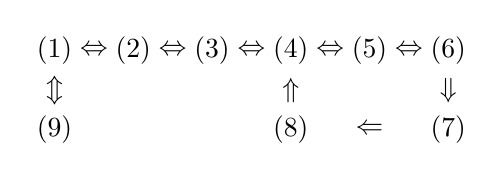
\begin{tikzpicture}[scale=1, transform shape]
       \tikzset{>=latex}
       \node[] (1) at (0,0) {$(1)$};
       \node[] (2) at (1,0) {$(2)$};
       \node[] (3) at (2,0) {$(3)$};
       \node[] (4) at (3,0) {$(4)$};
       \node[] (5) at (4,0) {$(5)$};
       \node[] (6) at (5,0) {$(6)$};
       \node[] (7) at (5,-1) {$(7)$};
       \node[] (8) at (3,-1) {$(8)$};
       \node[] (9) at (0,-1) {$(9)$};

       \node[] (1) at (0.5,0) {$\Leftrightarrow$};
       \node[] (1) at (1.5,0) {$\Leftrightarrow$};
       \node[] (1) at (2.5,0) {$\Leftrightarrow$};
       \node[] (1) at (3.5,0) {$\Leftrightarrow$};
       \node[] (1) at (4.5,0) {$\Leftrightarrow$};
       \node[] (1) at (5,-0.5) {$\Downarrow$};
       \node[] (1) at (4,-1) {$\Leftarrow$};
       \node[] (1) at (3,-0.5) {$\Uparrow$};
       \node[] (1) at (0,-0.5) {$\Updownarrow$};
   \end{tikzpicture}
   \end{center}
 \begin{proofnoend}
     (1), (2), (4), (5) and (6) are all equivalent.
     \bigskip

     \pause
     (6) $\Rightarrow$ (7) is clear. As for (7) $\Rightarrow$ (8), let $\vec{c}_j$ be one of the solution of $A \vec{x} = \vec{e}_j$.
     The
     \begin{align*}
	 A [\vec{c}_1,\cdots,\vec{c}_n] = [\vec{e}_1,\cdots,\vec{e}_n] = I
     \end{align*}
     Hence, (8) holds with $C=[\vec{c}_1,\cdots,\vec{c}_n]$.

     \bigskip


     \pause
     (1) $\Rightarrow$ (8) and (9): Using $C=A^{-1}$.

     \bigskip
     \pause
     (8) $\Rightarrow$ (4): Whenever $\vec{x}$ is a sol. i.e.,
     $A\vec{x}=\vec{0}$, then $\vec{x}=I\vec{x}=CA\vec{x}=C\vec{0}=\vec{0}$.
     Hence, $\vec{0}$ is the only solution. (4) holds true.

     \medskip
     \pause
     (9) $\Rightarrow$ (1): By reversing the roles of $A$ and $C$ and apply (8)
     to see that $C$ is invertible. Thus $A$ is the inverse of $C$, and hence $A$ is itself invertible.
 \myQED
 \end{proofnoend}
 }
 %-------------- end slide -------------------------------%}}}

%-------------- start slide -------------------------------%{{{ 33
 \frame{
 \begin{corollary}
     If $A$ and $B$ are $n\times n$ matrices such that $AB=I$, then
     $BA=I$.
     Furthermore, $A$ and $B$ are invertible, with $B=A^{-1}$ and
     $A=B^{-1}$.
 \end{corollary}
\vfill
 \begin{center}
   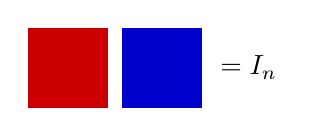
\begin{tikzpicture}[scale=1, transform shape]
       \tikzset{>=latex}
       \filldraw[red!80!black] (0,0) rectangle (1,1);
       \filldraw[blue!80!black] (1.2,0) rectangle (2.2,1);
       \node (a) at (2.8,0.5) {$= I_n$};
   \end{tikzpicture}
   \end{center}
   \pause
   \[\Downarrow\]
 \begin{center}
   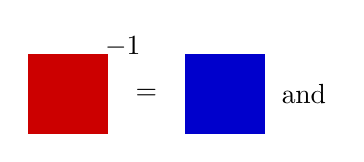
\begin{tikzpicture}[scale=1, transform shape]
       \tikzset{>=latex}
       \filldraw[red!80!black] (0,0) rectangle (1,1);
       \node (a) at (1.2,1.1) {$-1$};
       \node (a) at (1.5,0.5) {$=$};
       \filldraw[blue!80!black] (2,0) rectangle (3,1);
       \node (b) at (3.5,0.5) {and};
   \end{tikzpicture}
   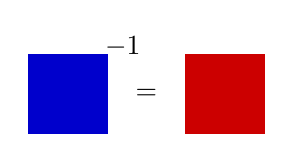
\begin{tikzpicture}[scale=1, transform shape]
       \tikzset{>=latex}
       \filldraw[blue!80!black] (0,0) rectangle (1,1);
       \node (a) at (1.2,1.1) {$-1$};
       \node (a) at (1.5,0.5) {$=$};
       \filldraw[red!80!black] (2,0) rectangle (3,1);
   \end{tikzpicture}
   \end{center}
 \pause
 \vfill
 \begin{remark}{Important Fact}
     In Corollary, it is essential that the matrices be square.
 \end{remark}
 }
%-------------- end slide -------------------------------%}}}

%-------------- start slide -------------------------------%{{{ 34
\frame{
\begin{theorem}
    If $A$ and $B$ are matrices such that $AB=I$ and $BA=I$, then
    $A$ and $B$ are square matrices (of the same size).
\end{theorem}
}
%-------------- end slide -------------------------------%}}}

%-------------- start slide -------------------------------%{{{ 35
\frame{
\begin{example}
    Let
    $A=\left[\begin{array}{rrr}
    1 & 1 & 0 \\ -1 & 4 & 1 \end{array}\right]
    \quad\text{and}\quad
    B=\left[\begin{array}{rr}
    1 & 0 \\ 0 & 0 \\ 1 & 1 \end{array}\right]$.
    \pause
    Then
    \[ AB=
	\left[\begin{array}{rrr}
	1 & 1 & 0 \\ -1 & 4 & 1 \end{array}\right]
	\left[\begin{array}{rr}
	1 & 0 \\ 0 & 0 \\ 1 & 1 \end{array}\right]
	\pause
	= \left[ \begin{array}{rr}
	1 & 0 \\ 0 & 1 \end{array} \right] =I_2
    \]
    \pause
    and
    \[ BA=
	\left[\begin{array}{rr}  1 & 0 \\ 0 &  0  \\ 1 & 1 \end{array}\right]
	\left[\begin{array}{rrr} 1 & 1 &  0 \\ -1 &  4 & 1 \end{array}\right]
	\pause
	= \left[ \begin{array}{rrr}
		1 & 1 & 0 \\
		0 & 0 & 0 \\
		0 & 5 & 1
	\end{array} \right] \neq I_3.
    \]
\end{example}
\pause
\vfill
\begin{remark}
    This example illustrates why ``an inverse'' of a non-square matrix
    doesn't make sense.
    If $A$ is $m\times n$ and $B$ is $n\times m$, where $m\neq n$,
    then even if $AB=I$, it will never be the case that $BA=I$.
\end{remark}
}
%-------------- end slide -------------------------------%}}}

\section[\textcolor{yellow}{}]{\textcolor{yellow}{Inverse of Transformations}}

%-------------- start slide -------------------------------%{{{ 36
\frame{
\frametitle{Inverse of Transformations}
\pause
\begin{definition}
    Suppose $T:\RR^n\rightarrow\RR^n$ and
    $S:\RR^n\rightarrow\RR^n$ are
     transformations such that
    for each $\vec{x}\in\RR^n$,
    \pause
    \[
	(S\circ T)(\vec{x}) = \vec{x} \quad\text{and}\quad
	(T\circ S)(\vec{x}) = \vec{x}.
    \]
    \pause
    Then $T$ and $S$ are \alert{invertible} transformations;
    \pause
    $S$ is called \alert{an inverse of $T$},
    \pause
    and $T$ is called \alert{an inverse of $S$}.
    \textcolor{blue}{(Geometrically, $S$ reverses the action of $T$,
    and $T$ reverses the action of $S$.)}
\end{definition}
\pause
\vfill
\begin{theorem}
    Let $T:\RR^n\rightarrow \RR^n$ be a matrix transformation induced
    by matrix $A$. Then we have:
    \begin{enumerate}
        \item $A$ is invertible if and only if $T$ has an inverse.
        \item In the case where $T$ has an inverse, the inverse is unique and is denoted $T^{-1}$.
        \item Furthermore, $T^{-1}:\RR^n\rightarrow \RR^n$ is induced by the matrix $A^{-1}$.
    \end{enumerate}
\end{theorem}
}
%-------------- end slide -------------------------------%}}}

%-------------- start slide -------------------------------%{{{ 37
\frame{
\begin{emptytitle}
    \textcolor{yellow}{Fundamental Identities relating $T$ and $T^{-1}$}
    \begin{enumerate}
	\item $T^{-1}\circ T = 1_{\RR^n}$
	\item $T\circ T^{-1} = 1_{\RR^n}$
    \end{enumerate}
\end{emptytitle}
}
%-------------- end slide -------------------------------%}}}

%-------------- start slide -------------------------------%{{{ 38
\frame{
\begin{example}
    Let $T : \mathbb{R}^2 \mapsto \mathbb{R}^2$ be a transformation given by
    \[
	T \left[
	\begin{array}{r}
	    x \\
	    y
	\end{array}\right]
	 =
	\left[
	\begin{array}{c}
	    x + y \\
	    y
	\end{array}
	\right]
    \]
    Then $T$ is a linear transformation induced by
    $A = \left[ \begin{array}{rr}
	1 & 1 \\
	0 & 1
    \end{array} \right]$.
    \pause

    Notice that the matrix $A$ is invertible. Therefore the transformation $T$ has an inverse, $T^{-1}$, induced by
    \[
    A^{-1} = \left[
    \begin{array}{rr}
	1 & -1 \\
	0 & 1
    \end{array} \right]
    \]
\end{example}
}
%-------------- end slide -------------------------------%}}}

%-------------- start slide -------------------------------%{{{ 39
\frame{
\begin{example}[continued]
    Consider the action of $T$ and $T^{-1}$:
    \pause
    \[
	T \left[ \begin{array}{r}
	    x \\
	    y
	\end{array} \right] = \left[ \begin{array}{rr}
	    1 & 1 \\
	    0 & 1
	\end{array} \right] \left[ \begin{array}{r}
	    x \\
	    y
	\end{array} \right]  = \left[ \begin{array}{c}
	    x + y \\
	    y
	\end{array} \right];
    \]
    \pause
    \[
	T^{-1} \left[ \begin{array}{c}
	    x + y \\
	    y
	\end{array}\right] = \left[ \begin{array}{rr}
	    1 & -1 \\
	    0 & 1
	\end{array} \right] \left[ \begin{array}{c}
	    x + y \\
	    y
	\end{array} \right] = \left[ \begin{array}{c}
	    x \\
	    y
	\end{array} \right].
    \]
    \pause
    Therefore,
    \[
	T^{-1} \left( T \left[ \begin{array}{c}
	    x \\
	    y
	\end{array} \right] \right) = \left[ \begin{array}{c}
	    x \\
	    y
	\end{array}
	\right].
    \]
    \myQED
\end{example}
}
%-------------- end slide -------------------------------%}}}

\end{document}
